\section{Key features} % (fold)
\begin{frame}\frametitle{Key features} 

\includegraphics[height=3cm]{sdcard.png}
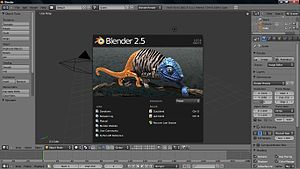
\includegraphics[height=3cm]{blender.jpg}
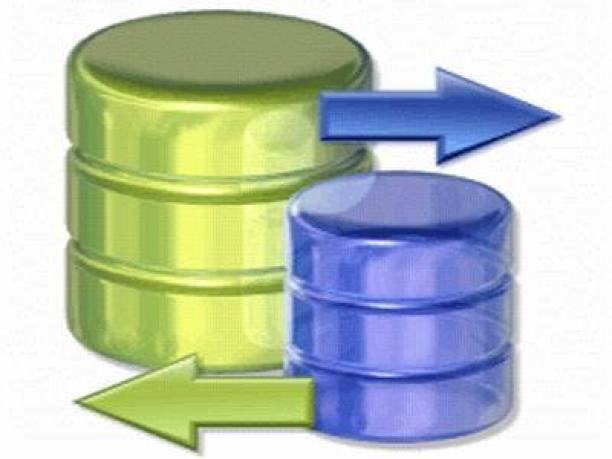
\includegraphics[height=3cm]{db.jpeg}
  \begin{block}{Simple - easy to use}
   Blender - simple creation \\
   Easy managing models \\
   No limitation with SDCard
  \end{block}
\end{frame}

\begin{frame}\frametitle{Time estimation} 
\begin{tabular}{| l || c | c |  c | c |}
\hline
Feature & Priority & Implemented & Hours* & Hours**\\
\hline
\hline
\textbf{Learning JNI} & high & YES &                 4 & {\bf ?} \\
\textbf{Exploring ndk samples} & high & YES &       12 &  {\bf ?} \\
\textbf{OpenGL demo} & high & YES &                  4 & {\bf ?} \\
\textbf{Running animation} & high & YES &           20 & {\bf ?} \\
\textbf{Loading OBJ definition} & high & YES &       6 &  {\bf ?} \\
\textbf{Select model} & high & YES &                 1 & {\bf ?} \\
\textbf{Full screen} & middle & YES &                3 &  {\bf ?} \\
\textbf{Screen saver} & middle & NO &                4 & {\bf ?} \\
\textbf{Binding colourising} & middle & NO &         4 & {\bf ?} \\
\textbf{Viewpoint manual} change & low & YES &       2 & {\bf ?} \\
\textbf{Docs \& refactoring} & middle & NO &         5 & {\bf ?} \\
\textbf{Design of XML} & high & NO &                15 & {\bf ?} \\
\hline
\textbf{Totally} &  & &                               80 & 172.5 \\
\hline
\end{tabular}
\end{frame}

\section{Screen shots} % (fold)
\begin{frame}\frametitle{Screen shot} 
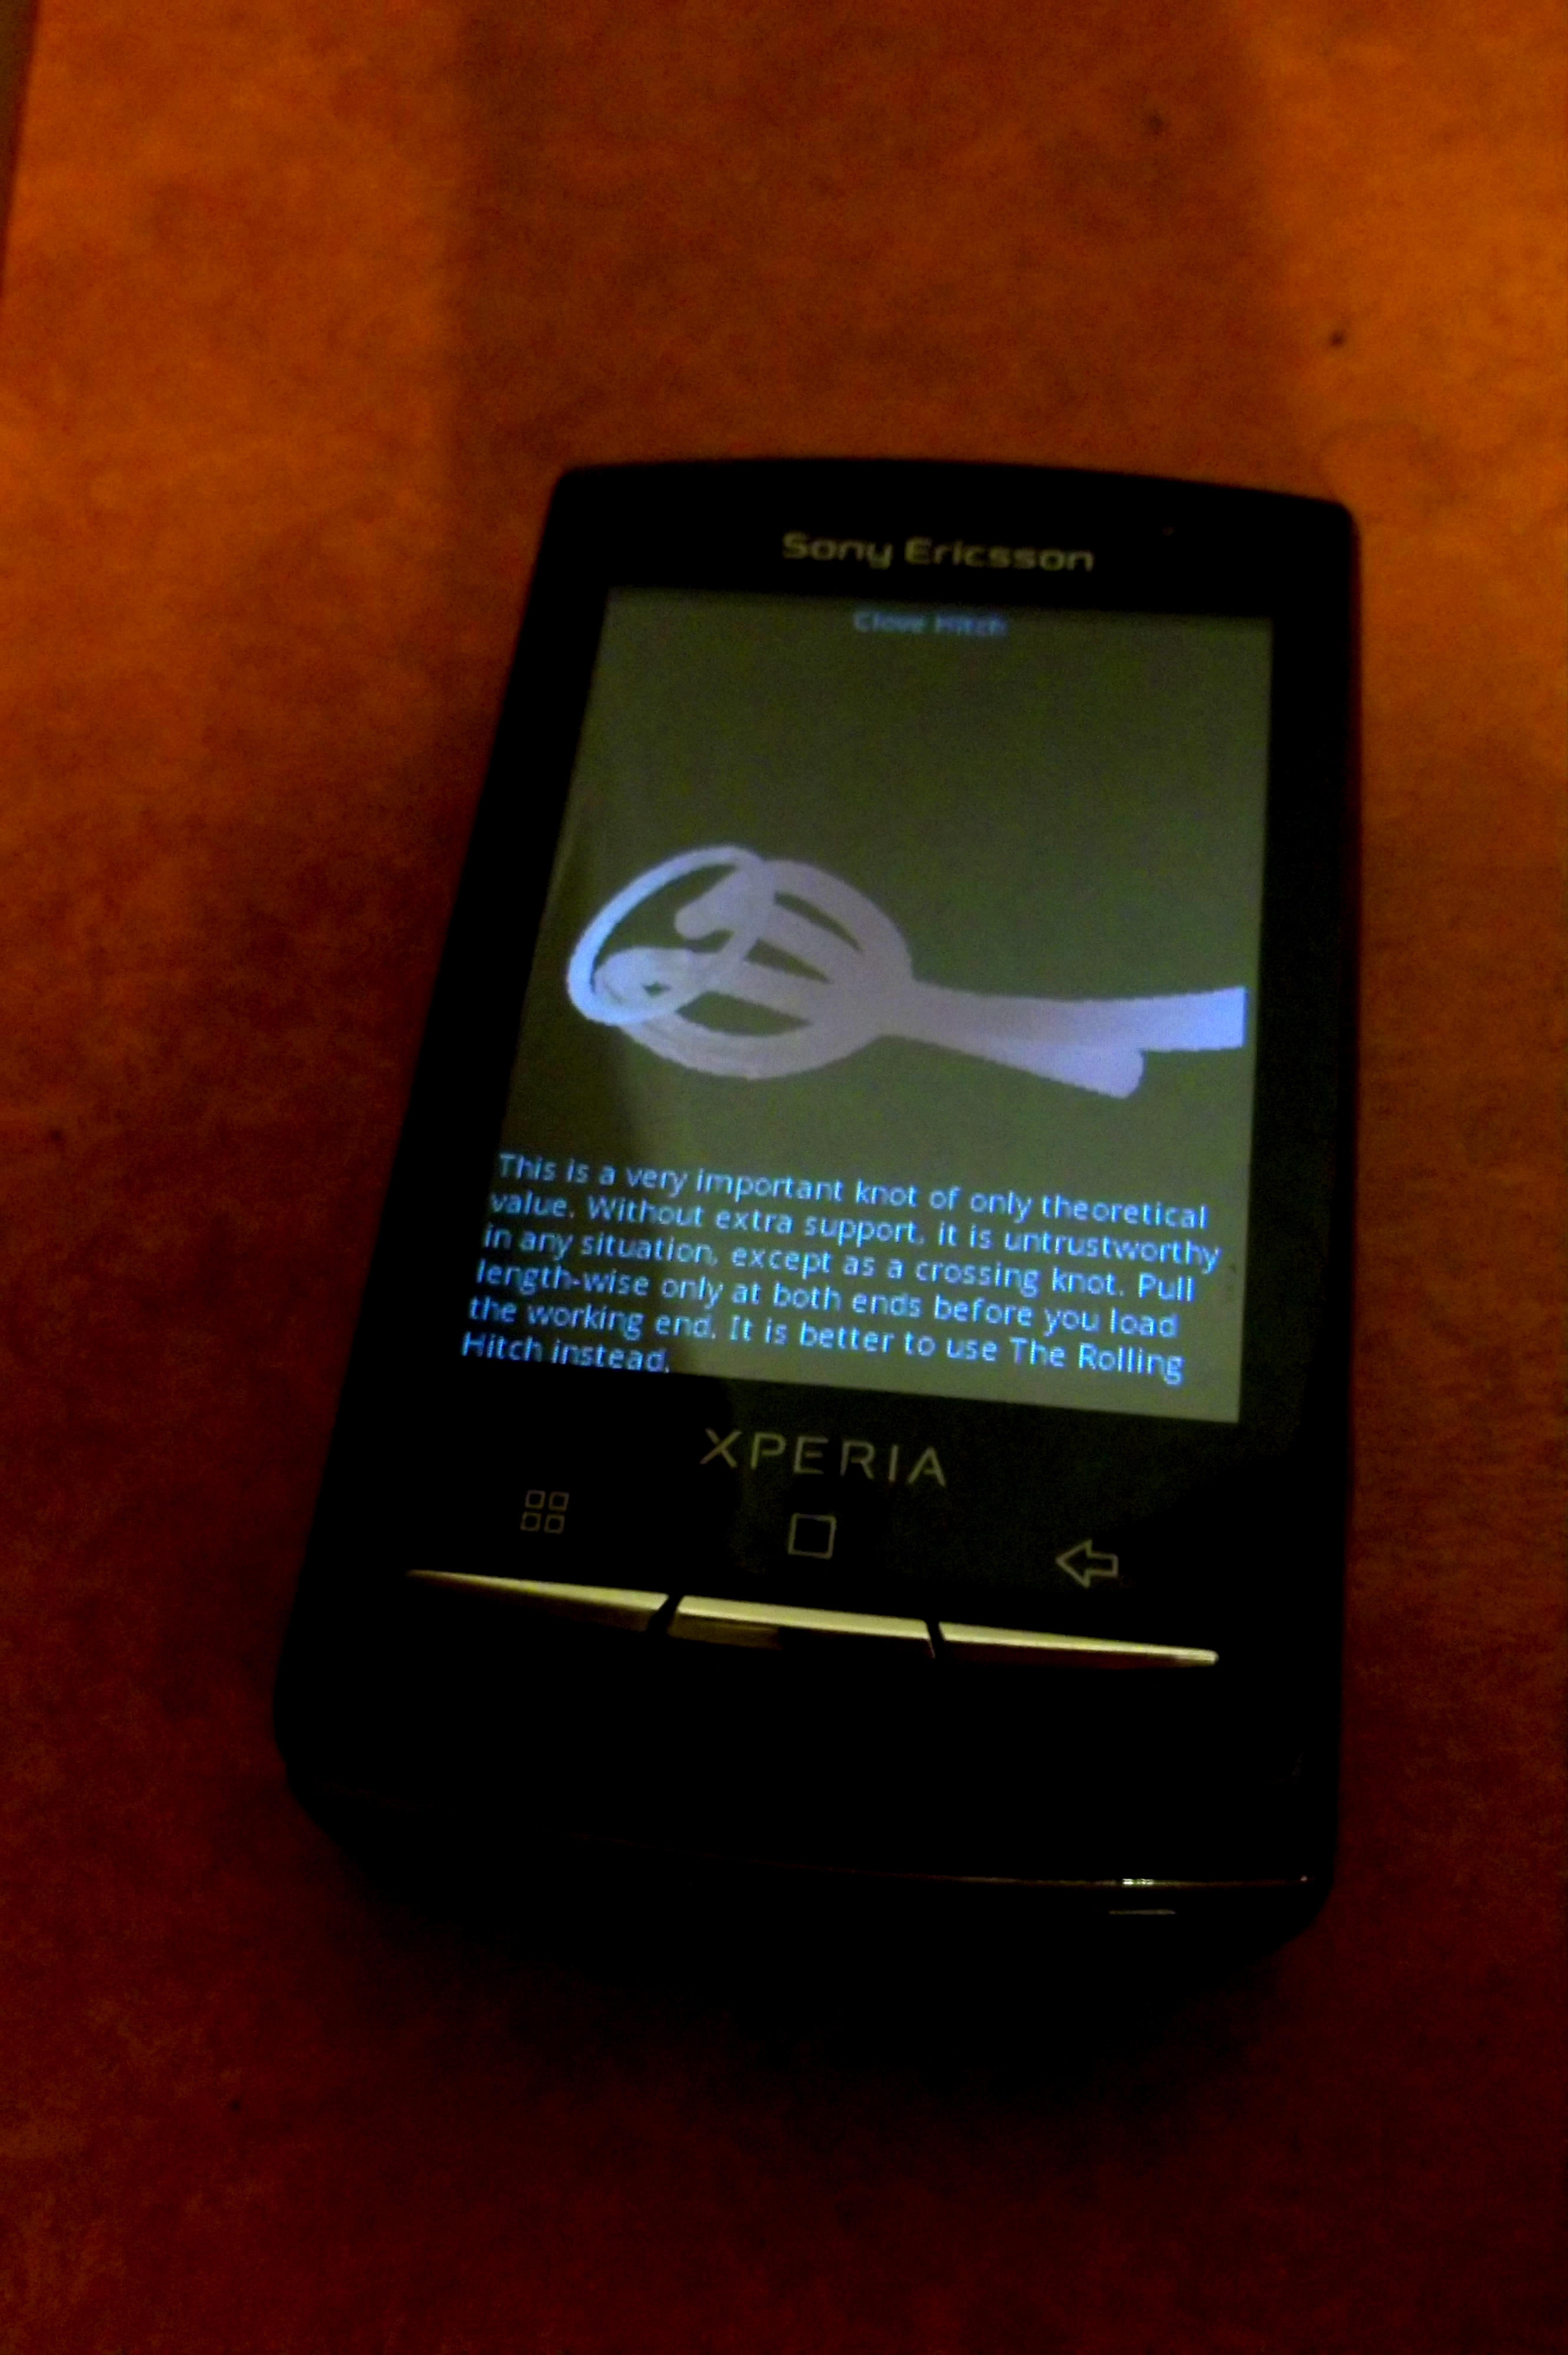
\includegraphics[height=8cm]{clove_hitch2.jpg}
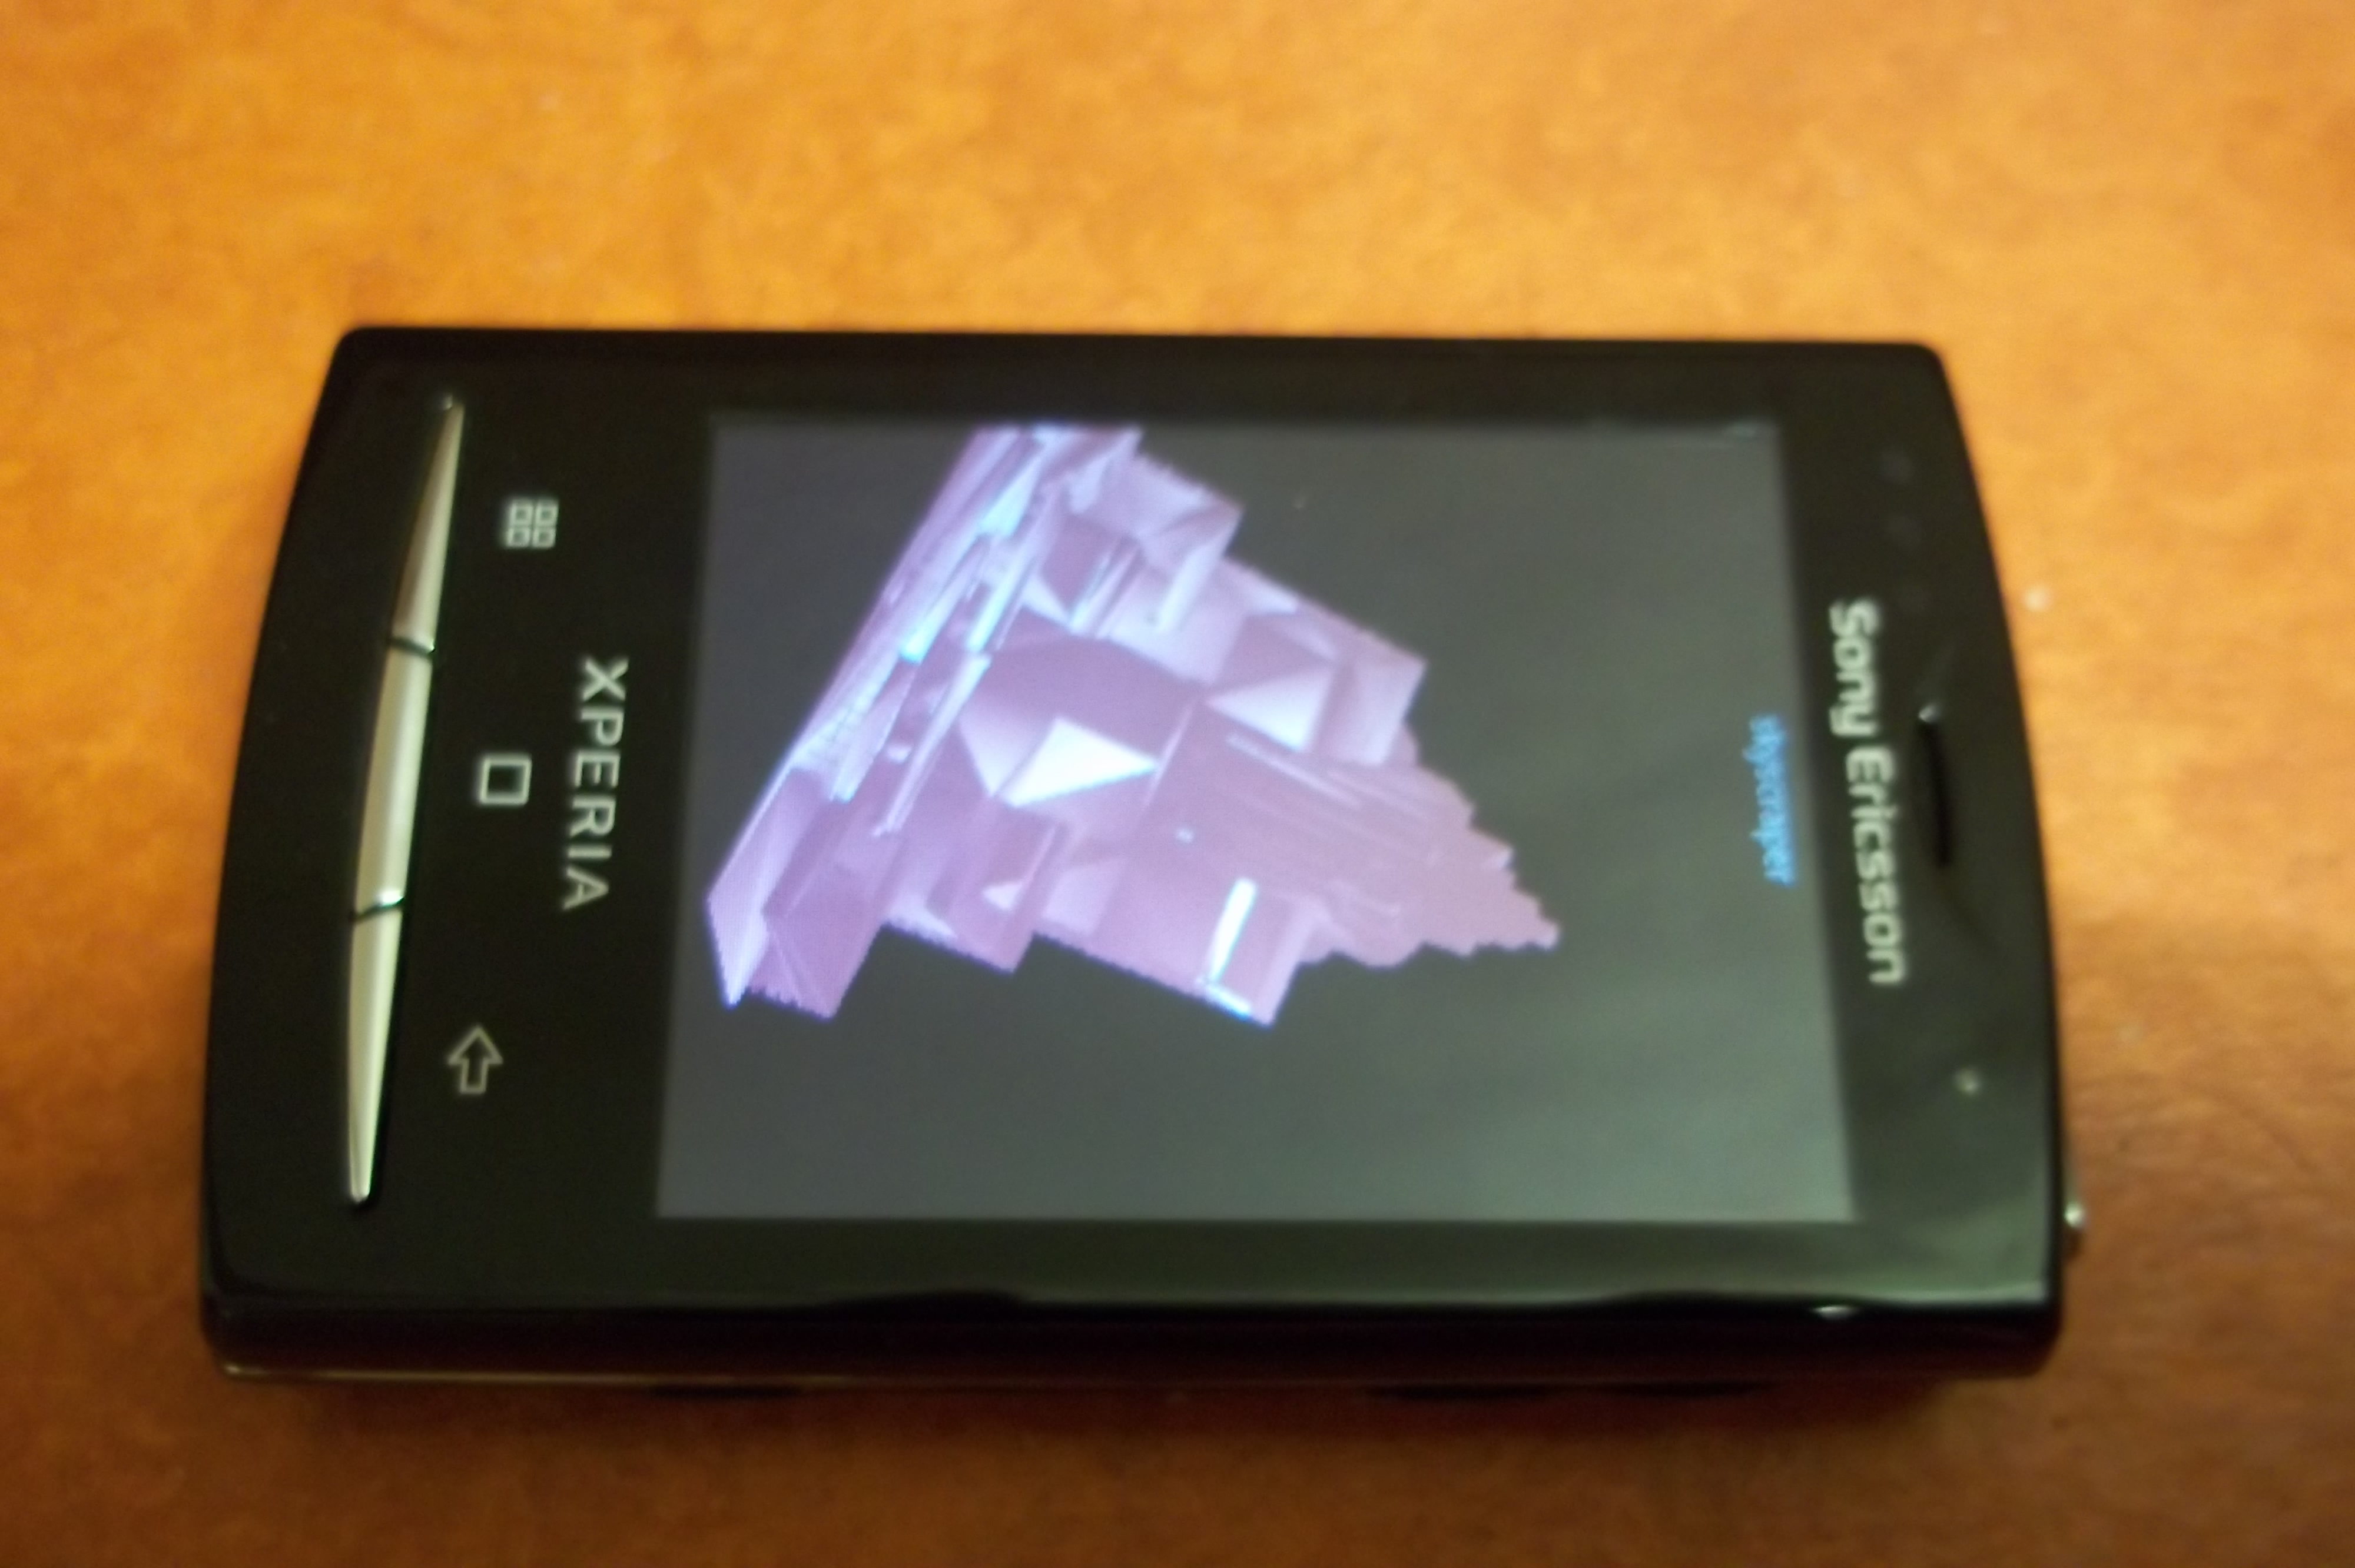
\includegraphics[height=8cm]{skyscraper.jpg}
\end{frame}

%\begin{frame} \frametitle{Bullet proofing} 
%\begin{enumerate}
%  \item Desired state
%  \item One color, no textures
%  \item Customizable view
%\end{enumerate}
%\end{frame}

\section{Workflow \& Inner structure} % (fold)
\begin{frame}\frametitle{Dream workflow} 
\begin{center}
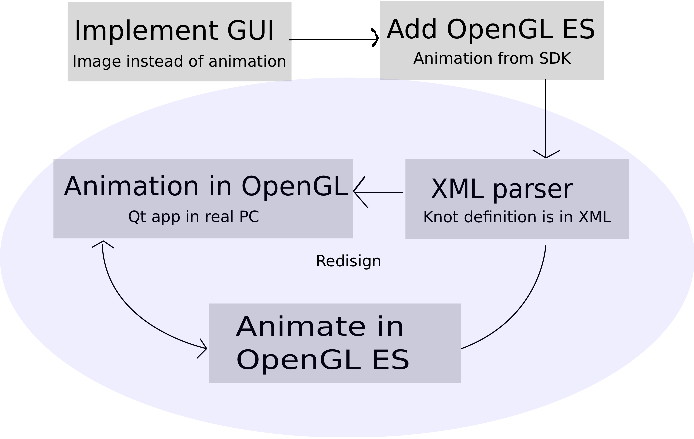
\includegraphics[height=8cm]{work_flow.png}
\end{center}
\end{frame}

\begin{frame}\frametitle{X11 linux application} 
\begin{center}
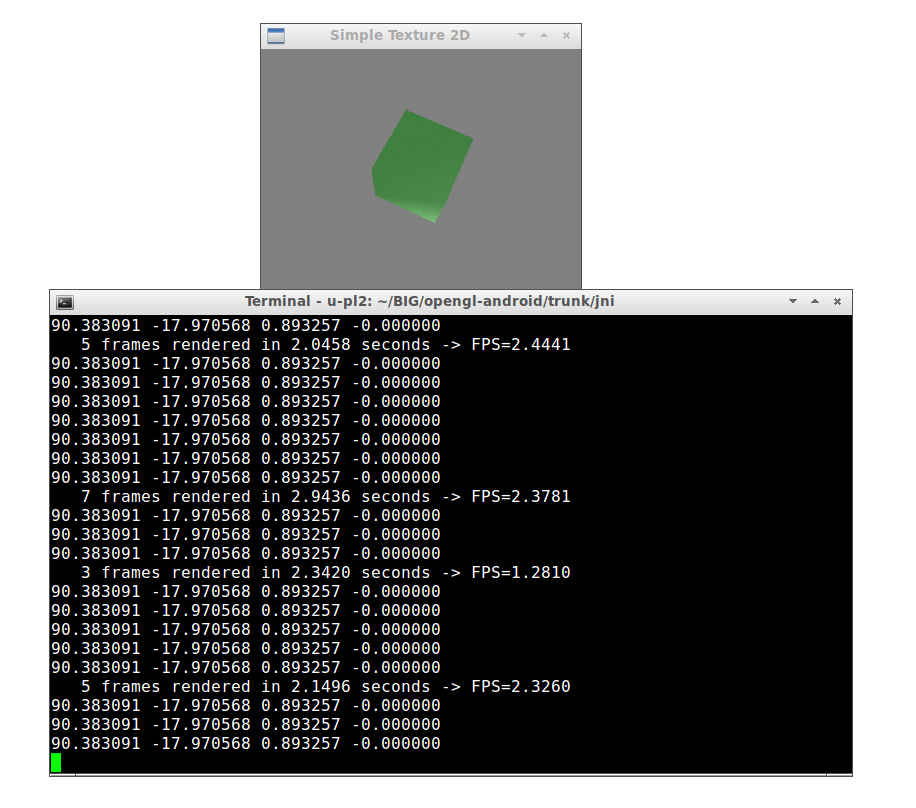
\includegraphics[height=8cm]{x11renderer.png}
\end{center}
\end{frame}

\begin{frame}\frametitle{Inner structure} 
\begin{center}
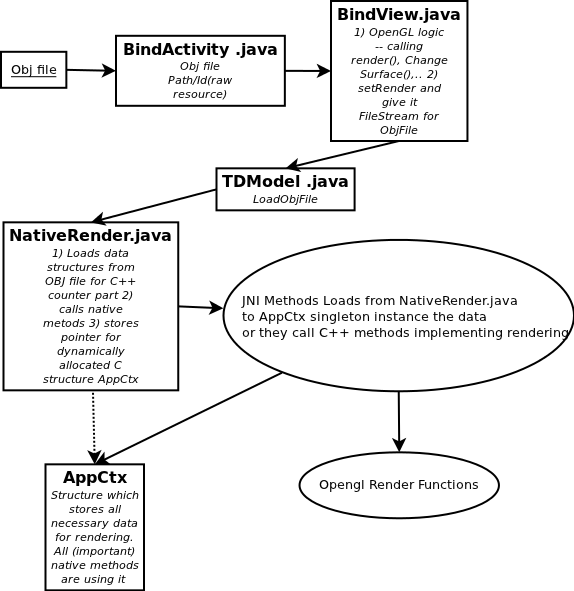
\includegraphics[height=8cm]{structure.png}
\end{center}
\end{frame}


\section{Evaluation} % (fold)
\begin{frame}\frametitle{Time estimation} 
\begin{tabular}{| l || c | c |  c | c |}
\hline
Feature & Priority & Implemented & Hours* & Hours**\\
\hline
\hline
\textbf{Learning JNI} & high & YES &                 4 & 51.5\\
\textbf{Exploring ndk samples} & high & YES &       12 & 11.5\\
\textbf{OpenGL demo} & high & YES &                  4 & 25\\
\textbf{Running animation} & high & YES &           20 & 40\\
\textbf{Loading OBJ definition} & high & YES &       6 &  8.5\\
\textbf{Select model} & high & YES &                 1 & 10\\
\textbf{Full screen} & middle & YES &                3 &  0\\
\textbf{Screen saver} & middle & NO &                4 &  -\\
\textbf{Binding colourising} & middle & NO &         4 & -\\
\textbf{Viewpoint manual} change & low & YES &       2 & 5\\
\textbf{Docs \& refactoring} & middle & NO &         5 & 20\\
\textbf{Design of XML} & high & NO &                15 & 1\\
\hline
\textbf{Totally} & & &                                80 & 172.5 \\
\hline
\end{tabular}
\end{frame}

\begin{frame}\frametitle{Summary} 
\begin{itemize}
    \item New technologies: Java, JNI, Android, Eclipse, OpenGLES 2.0
    \item Hard to debug string transfers Java/JNI/C++/GLSL
    \item Efficient
    \item Not as good as paid application
    \item Good base for future work
\end{itemize}
\end{frame}


\begin{frame}\frametitle{Questions?} 
\begin{center}

\includegraphics[height=8cm]{android_thank_you.jpg}
\end{center}
\end{frame}
